\ifdefined\ishandout
  \documentclass[handout,landscape]{beamer} 
\else
  \documentclass[landscape]{beamer}
\fi

%\hypersetup{pdfpagemode=FullScreen} %Enabling this option will cause the slides to go full-screen on opening

\mode<handout>
{
  \usepackage{pgf}
  \usepackage{pgfpages}

\pgfpagesdeclarelayout{6 on 1 boxed}
{
  \edef\pgfpageoptionheight{\the\paperheight} 
  \edef\pgfpageoptionwidth{\the\paperwidth}
  \edef\pgfpageoptionborder{0pt}
}
{
  \pgfpagesphysicalpageoptions
  {%
    logical pages=6,%
    physical height=\pgfpageoptionheight,%
    physical width=\pgfpageoptionwidth%
  }
  \pgfpageslogicalpageoptions{1}
  {%
    border code=\pgfsetlinewidth{2pt}\pgfstroke,%
    border shrink=\pgfpageoptionborder,%
    resized width=.5\pgfphysicalwidth,%
    resized height=.5\pgfphysicalheight,%
    center=\pgfpoint{.25\pgfphysicalwidth}{.833\pgfphysicalheight}%
  }%
  \pgfpageslogicalpageoptions{2}
  {%
    border code=\pgfsetlinewidth{2pt}\pgfstroke,%
    border shrink=\pgfpageoptionborder,%
    resized width=.5\pgfphysicalwidth,%
    resized height=.5\pgfphysicalheight,%
    center=\pgfpoint{.75\pgfphysicalwidth}{.833\pgfphysicalheight}%
  }%
  \pgfpageslogicalpageoptions{3}
  {%
    border code=\pgfsetlinewidth{2pt}\pgfstroke,%
    border shrink=\pgfpageoptionborder,%
    resized width=.5\pgfphysicalwidth,%
    resized height=.5\pgfphysicalheight,%
    center=\pgfpoint{.25\pgfphysicalwidth}{.5\pgfphysicalheight}%
  }%
  \pgfpageslogicalpageoptions{4}
  {%
    border code=\pgfsetlinewidth{2pt}\pgfstroke,%
    border shrink=\pgfpageoptionborder,%
    resized width=.5\pgfphysicalwidth,%
    resized height=.5\pgfphysicalheight,%
    center=\pgfpoint{.75\pgfphysicalwidth}{.5\pgfphysicalheight}%
  }%
  \pgfpageslogicalpageoptions{5}
  {%
    border code=\pgfsetlinewidth{2pt}\pgfstroke,%
    border shrink=\pgfpageoptionborder,%
    resized width=.5\pgfphysicalwidth,%
    resized height=.5\pgfphysicalheight,%
    center=\pgfpoint{.25\pgfphysicalwidth}{.167\pgfphysicalheight}%
  }%
  \pgfpageslogicalpageoptions{6}
  {%
    border code=\pgfsetlinewidth{2pt}\pgfstroke,%
    border shrink=\pgfpageoptionborder,%
    resized width=.5\pgfphysicalwidth,%
    resized height=.5\pgfphysicalheight,%
    center=\pgfpoint{.75\pgfphysicalwidth}{.167\pgfphysicalheight}%
  }%
}


  \pgfpagesuselayout{6 on 1 boxed}[letterpaper, border shrink=5mm]
  \nofiles
}

\usepackage{listings}
\usepackage{multimedia}
\usepackage[normalem]{ulem}
\usepackage{ifthen}

\usetheme{Warsaw} 
\usecolortheme{seahorse}
\useoutertheme{infolines} 

\setbeamertemplate{blocks}[rounded][shadow=true] 

\author{Joe Fields}
\title{Introduction to Proof} 

\date{Lecture 23 (GIAM \S 4.4) \newline }
\institute[SCSU]{ {\tt fieldsj1@southernct.edu} }


\newlength{\cwidth}
\newcommand{\cents}{\settowidth{\cwidth}{c}%
\divide\cwidth by2
\advance\cwidth by-.1pt
c\kern-\cwidth
\vrule width .1pt depth.2ex height1.2ex
\kern\cwidth}

\newcommand{\sageprompt}{ {\tt sage$>$} }
\newcommand{\tab}{\rule{20pt}{0pt}}
\newcommand{\blnk}{\rule{1.5pt}{0pt}\rule{.4pt}{1.2pt}\rule{9pt}{.4pt}\rule{.4pt}{1.2pt}\rule{1.5pt}{0pt}}
\newcommand{\suchthat}{\; \rule[-3pt]{.25pt}{13pt} \;}
\newcommand{\divides}{\!\mid\!}
\newcommand{\tdiv}{\; \mbox{div} \;}
\newcommand{\restrict}[2]{#1 \,\rule[-4pt]{.125pt}{14pt}_{\,#2}}
\newcommand{\lcm}[2]{\mbox{lcm} (#1, #2)}
\renewcommand{\gcd}[2]{\mbox{gcd} (#1, #2)}
\newcommand{\Naturals}{{\mathbb N}}
\newcommand{\Integers}{{\mathbb Z}}
\newcommand{\Znoneg}{{\mathbb Z}^{\mbox{\tiny noneg}}}
\newcommand{\Enoneg}{{\mathbb E}^{\mbox{\tiny noneg}}}
\newcommand{\Qnoneg}{{\mathbb Q}^{\mbox{\tiny noneg}}}
\newcommand{\Rnoneg}{{\mathbb R}^{\mbox{\tiny noneg}}}
\newcommand{\Rationals}{{\mathbb Q}}
\newcommand{\Reals}{{\mathbb R}}
\newcommand{\Complexes}{{\mathbb C}}
%\newcommand{\F2}{{\mathbb F}_{2}}
\newcommand{\relQ}{\mbox{\textsf Q}}
\newcommand{\relR}{\mbox{\textsf R}}
\newcommand{\nrelR}{\mbox{\raisebox{1pt}{$\not$}\rule{1pt}{0pt}{\textsf R}}}
\newcommand{\relS}{\mbox{\textsf S}}
\newcommand{\relA}{\mbox{\textsf A}}
\newcommand{\Dom}[1]{\mbox{Dom}(#1)}
\newcommand{\Cod}[1]{\mbox{Cod}(#1)}
\newcommand{\Rng}[1]{\mbox{Rng}(#1)}

\DeclareMathOperator\caret{\raisebox{1ex}{$\scriptstyle\wedge$}}

\newtheorem*{defi}{Definition}
\newtheorem*{exer}{Exercise}
\newtheorem{thm}{Theorem}[section]
\newtheorem*{thm*}{Theorem}
\newtheorem{lem}[thm]{Lemma}
\newtheorem{cor}{Corollary}
\newtheorem{conj}{Conjecture}

\renewenvironment{proof}%
{\begin{quote} \emph{Proof:} }%
{\rule{0pt}{0pt} \newline \rule{0pt}{15pt} \hfill Q.E.D. \end{quote}}


\newcommand{\vs}{\rule{0pt}{12pt}}
\newcommand{\notimplies}{\;\not\!\!\!\implies}

\AtBeginSection[]
{
 \begin{frame}{Table of Contents} 
  \tableofcontents[currentsection]
 \end{frame}
}

%%%% SAVE %%%%
%{ %magic to get a full screen image...
%\setbeamertemplate{navigation symbols}{}  % hide navigation buttons 
%\setbeamertemplate{background canvas}{\centerline{\includegraphics 
%	[height=\paperheight]{Cantor_4.jpeg}}}
%\begin{frame}[plain]
%\rule{0pt}{0pt}
%\end{frame} 
%} %end of magic


\begin{document}

\begin{frame}[plain]
  \titlepage
\end{frame}

\section{some additional comments on \S 4.3}

\begin{frame}{double inclusion proofs}
\begin{itemize}
\item A good way to proceed to show that $A=B$, is to seperately prove that $A \subseteq B$ and also that $B \subseteq A$.  \pause
\item A good way to do {\em that} is known as ``element chasing.'' \pause
\begin{itemize}
\item Suppose $x \in A$ and argue until you conclude that $x \in B$. \pause 
\item Then turn it around and show that $x \in B$ implies $x \in A$.
\end{itemize}
\item Let's illustrate this approach by proving one of DeMorgan's laws in this style.
\end{itemize}
\end{frame}

\begin{frame}{DeMorgan's}
\begin{thm*}
For all sets $A$ and $B$ contained in a universal set $U$,
$ \overline{A \cup B} \; = \; \overline{A} \cap \overline{B}.$
\end{thm*}
{\em Proof:}
\begin{quote}
First we will show that $\overline{A \cup B} \; \subseteq \; \overline{A} \cap \overline{B} $.\newline
Towards that end, suppose $x \in \overline{A \cup B}$. 
\begin{align*}
 &      & x \in \overline{A \cup B} \rule{48pt}{0pt} & \mbox{Given} & \\
 & \implies & \lnot (x \in (A \cup B)) \rule{48pt}{0pt} & \mbox{Def.\ of complement} & \\
 & \implies & \lnot (x \in A \, \lor \, x \in B) \rule{48pt}{0pt} & \mbox{Def.\ of union} & \\
 & \implies & \lnot (x \in A) \, \land  \, \lnot (x \in B) \rule{48pt}{0pt} & \mbox{disjunctive version of DeMorgan's law } & \\
 & \implies &  (x \in \overline{A}) \, \land  \, (x \in \overline{B}) \rule{48pt}{0pt} & \mbox{Def.\ of complement} & \\
 & \implies &  x \in ( \overline{A} \, \cap \, \overline{B}) \rule{48pt}{0pt} & \mbox{Def.\ of intersection} & \\
\end{align*}

(continued)

\end{quote}
\end{frame}

\begin{frame}{continued}
Next we will show that $\overline{A} \cap \overline{B} \; \subseteq \; \overline{A \cup B}$.
Suppose $x \in \overline{A} \cap \overline{B}$.
\begin{align*}
 &          &  x \in ( \overline{A} \, \cap \, \overline{B}) \rule{48pt}{0pt} & \mbox{Given} & \\
 & \implies &  (x \in \overline{A}) \, \land  \, (x \in \overline{B}) \rule{48pt}{0pt} & \mbox{Def.\ of intersection} & \\
 & \implies & \lnot (x \in A) \, \land  \, \lnot (x \in B) \rule{48pt}{0pt} & \mbox{Def.\ of complement } & \\
 & \implies & \lnot (x \in A \, \lor \, x \in B) \rule{48pt}{0pt} & \mbox{disjunctive version of DeMorgan's law} & \\
 & \implies & \lnot (x \in (A \cup B)) \rule{48pt}{0pt} & \mbox{Def.\ of union} & \\
 & \implies & x \in \overline{A \cup B} \rule{48pt}{0pt} & \mbox{Def.\ of complement} & \\
\end{align*}

\rule{0pt}{0pt} \hfill {\em Q.E.D} 

\end{frame}

\section{Jordan curves}


\begin{frame}{intro}
\begin{itemize}
\item A {\em Jordan curve} is a simple closed curve in the plane. \pause
\item A mapping from $[0,1]$ into the plane where $f(0) = f(1)$ is called closed.\pause
\item Simple means that $0$ and $1$ are the only such values: \pause \newline
\[ \forall a, b \in \Reals, \; 0<a<b<1 \, \implies \, f(a) \neq f(b). \] \pause
\item The mapping $f$ also must be continuous.  \pause
\item On an intuitive basis this just means that you can draw the 
curve without lifting your pencil from the paper.\pause
\item Examples
\end{itemize}
\end{frame}

\begin{frame}{the Jordan curve theorem}
\begin{itemize}
\item A Jordan curve divides the plane into two regions.\pause
\item You can also draw a Jordan curve on a sphere, but the two regions may be harder to distinguish. \pause
\item Think of how the equator divides the Earth into northern and southern hemispheres. \pause
\item Break for humor. \pause
\item In the plane, one region will always be unbounded.  Typically we call that the outside.
\end{itemize}
\end{frame}

\begin{frame}{CMC 2010}
\centerline{Problem 3 on the 2010 Collegiate Math Competition}

 (This problem was dedicated to the memory of Martin Gardner.)  

The point labeled $A$ is inside a simple closed curve that is partially hidden under a piece of paper with a rectangular hole in it. (See the diagram on the next slide.)  Is it possible to say whether the point labeled $B$ is also inside the curve?  If so, which is it, inside or outside?

\end{frame}

%%% SAVE %%%%
{ %magic to get a full screen image...
\setbeamertemplate{navigation symbols}{}  % hide navigation buttons 
\setbeamertemplate{background canvas}{\centerline{\includegraphics 
	[height=\paperheight]{simple_closed_curve.pdf}}}
\begin{frame}[plain]
\rule{0pt}{0pt}
\end{frame} 
} %end of magic

%%% SAVE %%%%
{ %magic to get a full screen image...
\setbeamertemplate{navigation symbols}{}  % hide navigation buttons 
\setbeamertemplate{background canvas}{\centerline{\includegraphics 
	[height=\paperheight]{simple_closed_curve_transparent.pdf}}}
\begin{frame}[plain]
\rule{0pt}{0pt}
\end{frame} 
} %end of magic


\section{Venn diagrams}

\begin{frame}{getting started}
\begin{itemize}
\item A Venn diagram is a collection of $n$ Jordan curves that divide the plane into $2^n$ regions. \pause
\item Let's start with $n=2$. \pause

\vspace{.2in}

\includegraphics[scale=.75]{general_Venn.pdf} \pause

\vspace{.2in}

\item The universal set $U$ is the big rectangle that holds the other sets.

\end{itemize}
\end{frame}

\begin{frame}{a few notes}
\begin{itemize}
\item Notice that there are $2^2=4$ regions that correspond to $A \cap B$, $A \cap \overline{B}$, $\overline{A} \cap B$ and $\overline{A} \cap \overline{B}$. \pause
\item This is related to the disjunctive normal form we saw in Chapter 2. \pause
\item There's no ``Michigan effect'' (exclaves) \pause
\item A Google Earth break. \pause
\item In general we'll have every possible combination of complemented or not which is why there are $2^n$ regions. \pause
\item Don't forget to count the outside as a region!
\end{itemize}
\end{frame}

\begin{frame}{using Venn}
\begin{itemize}
\item We put the emptyset symbol ($\emptyset$) in a region to indicate that no elements are actually present in that region.\pause
\item This allows us to use the general position Venn diagram to deal with special cases. \pause
\item $A$ and $B$ disjoint. \pause
\item $A \subseteq B$. 
\end{itemize}
\end{frame}

\begin{frame}{n=3}
\begin{itemize}
\item 3 sets

\vspace{.2in}

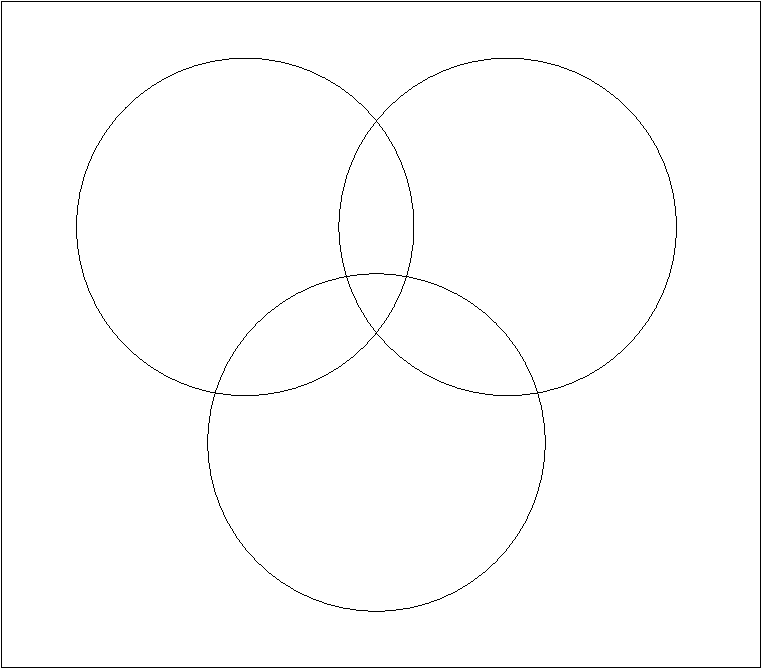
\includegraphics{3set_Venn.pdf}

\vspace{.2in}

\end{itemize}
\end{frame}

\begin{frame}{no more circles}
\begin{itemize}
\item After 3 set Venn diagrams you can't get the job done with circles. \pause
\item 4 sets w/ ellipses (GIAM page 190)\pause
\item Rectilinear curves are the sort of thing you might produce with an etch-a-sketch. \pause \newline
(Do kids still play with those?) \pause
\item 5 sets w/ ``lightbulbs'' (wrongness of the 5 sets w/ circles that shows up 1st on Google)
\end{itemize}
\end{frame}


\end{document}
